\documentclass[../main.tex]{subfiles}
 
\begin{document}

\section{Összefoglalás: Elkészült eszköz értékelése és költségterv számolása}
    \subsection{Az elkészült eszköz értékelése}
        Összesen 5 eszközhöz elegendő alkatrészt rendeltem meg, amelyekből 3 kész LED sor vezérlő került sikeresen elkészítésre. Kettő javított verziójú és egy pedig az eredetileg elkészített NYÁK-kal működik. Mind a három egység stabil, üzembiztos viselkedést mutat. Az egyik egység az otthoni teraszunkra (\ref{fig:pic_terasz}. ábra), a másik a kollégiumi szobába került felszerelésre. A harmadik egység tartalékként működik. Az eszköz tesztelve lett akkumulátorról is, egy Halloween-i jelmez kellékeként. Három cellás (12V-os), 2200mAh-s LiPo (Lítium Polimer) akkumulátorról üzemeltetve 5 órán keresztül működött. Az elkészült Android-os alkalmazással és LED sor vezérlővel a feladat célkitűzéseit teljesítettem.
    
        \begin{figure}[h!]
            \centering
                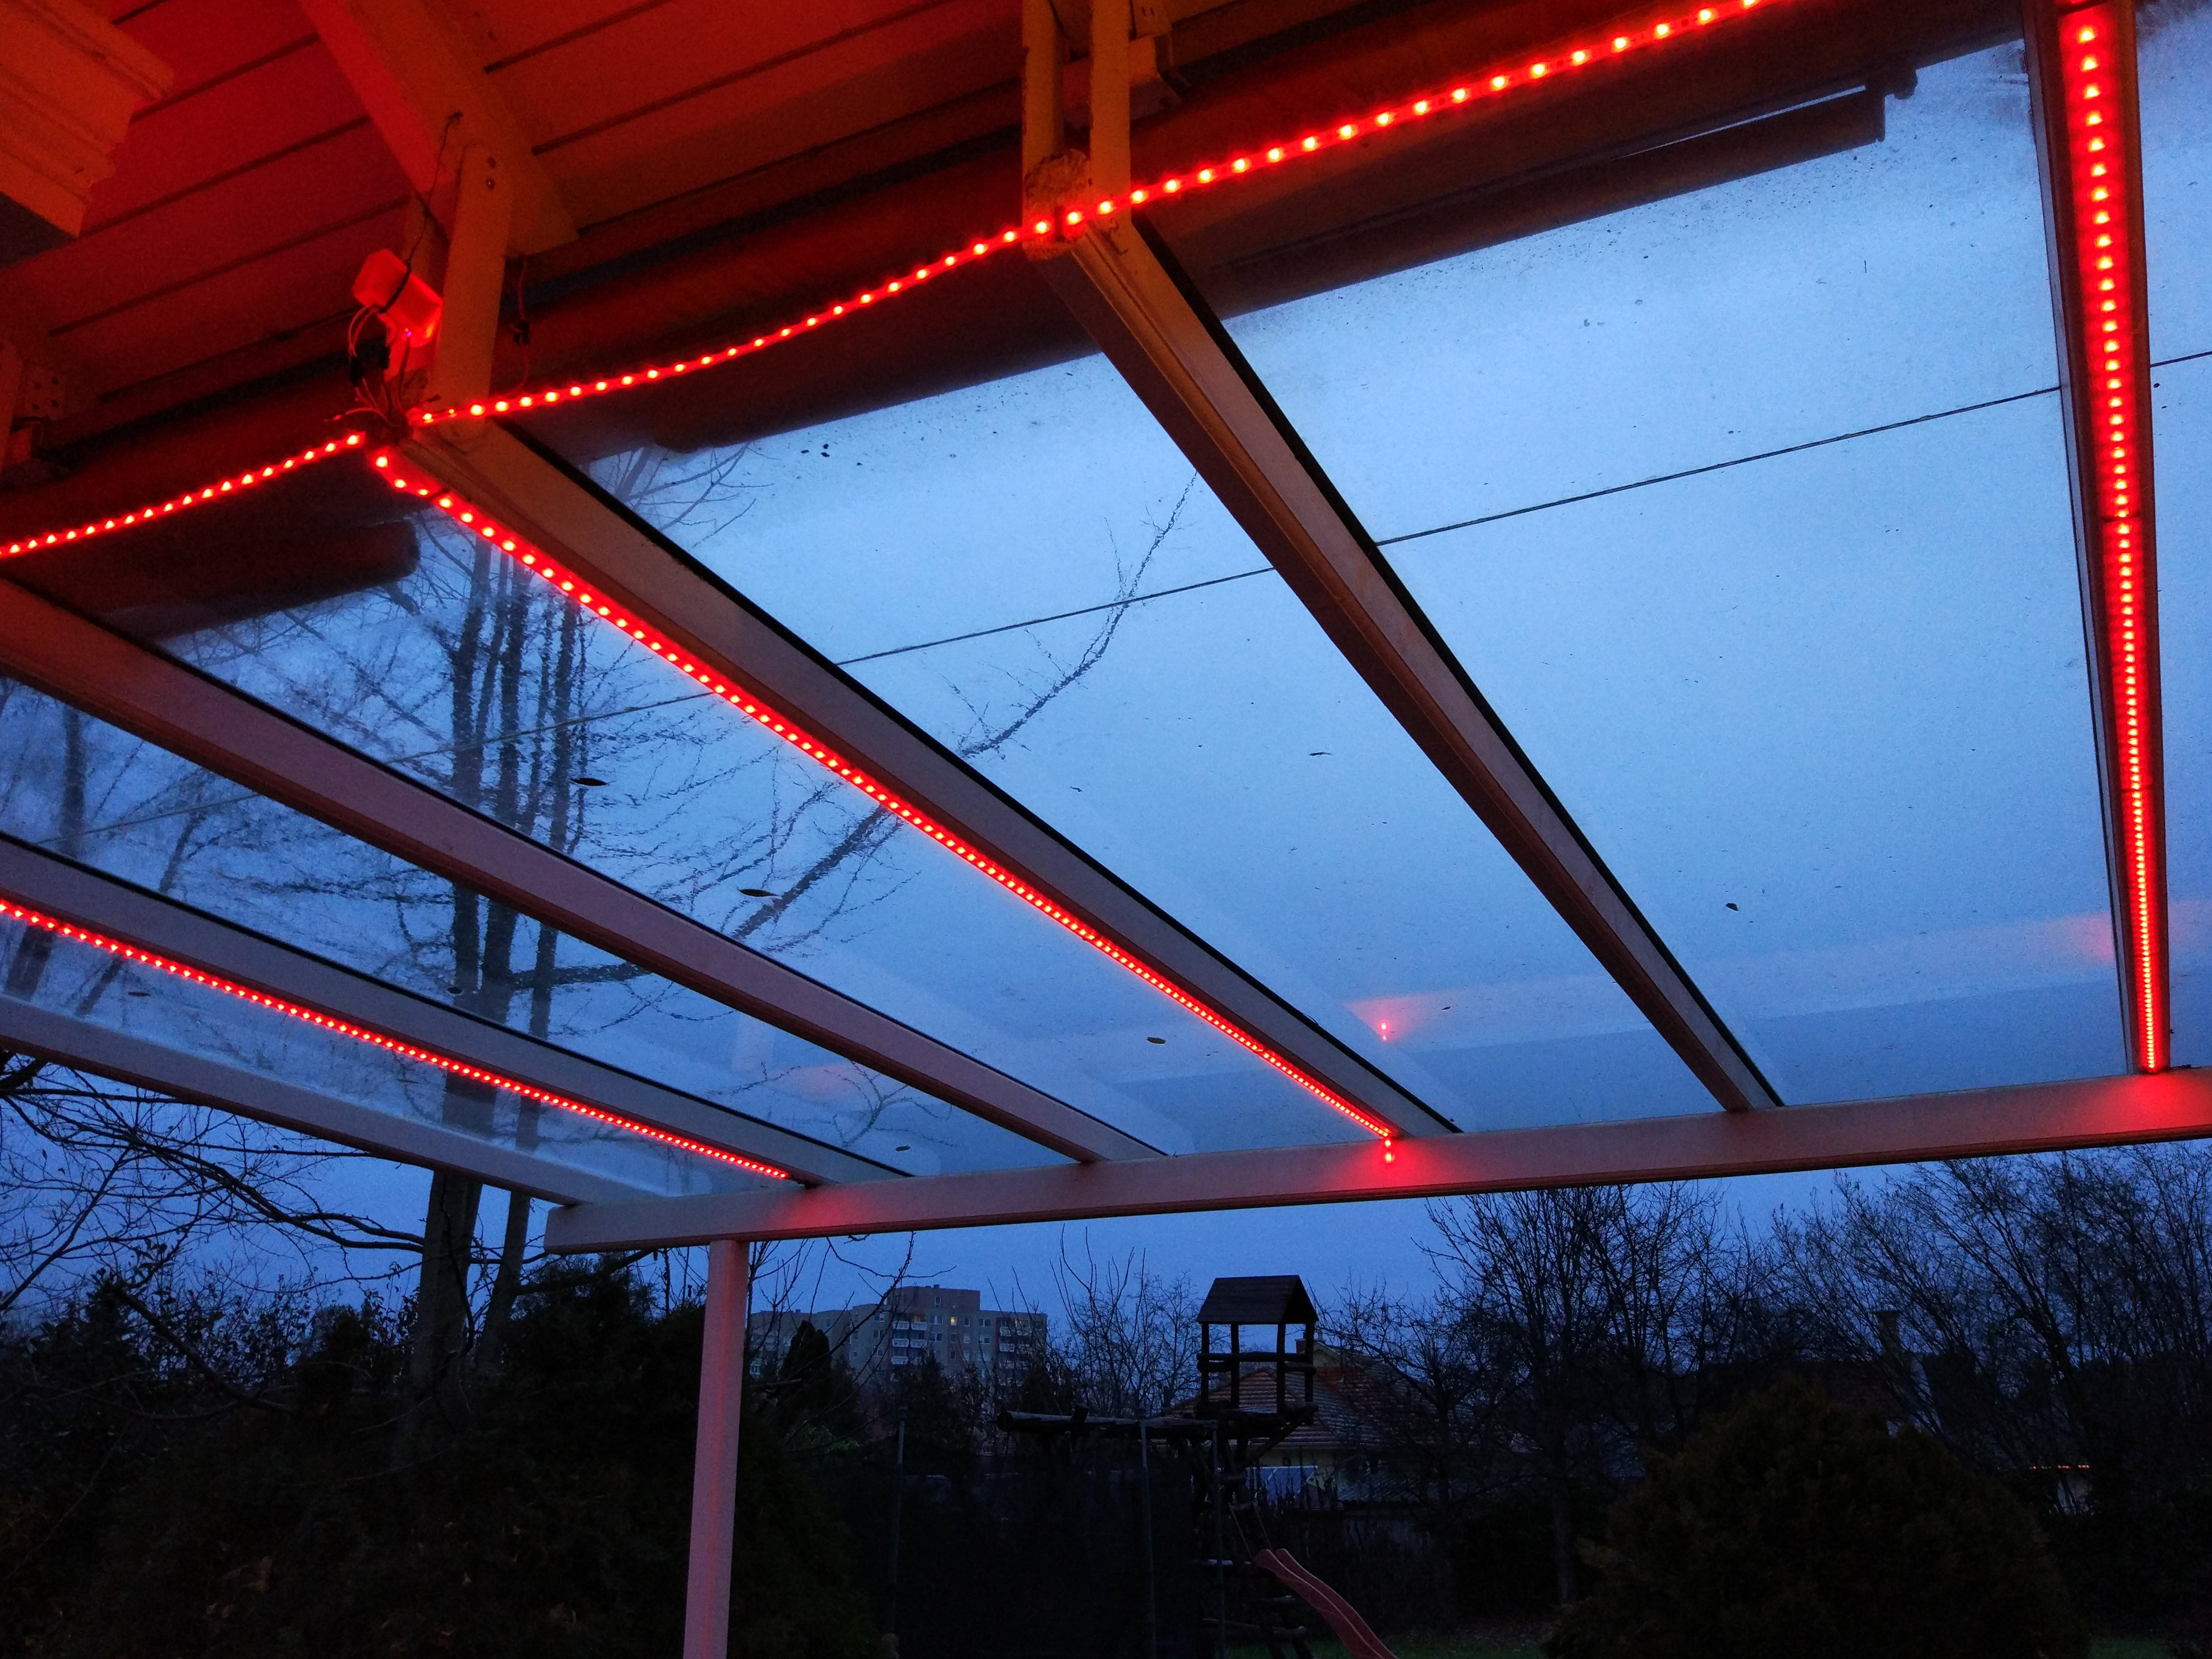
\includegraphics[height=3.8cm]{resources/alk_res/1_red}
                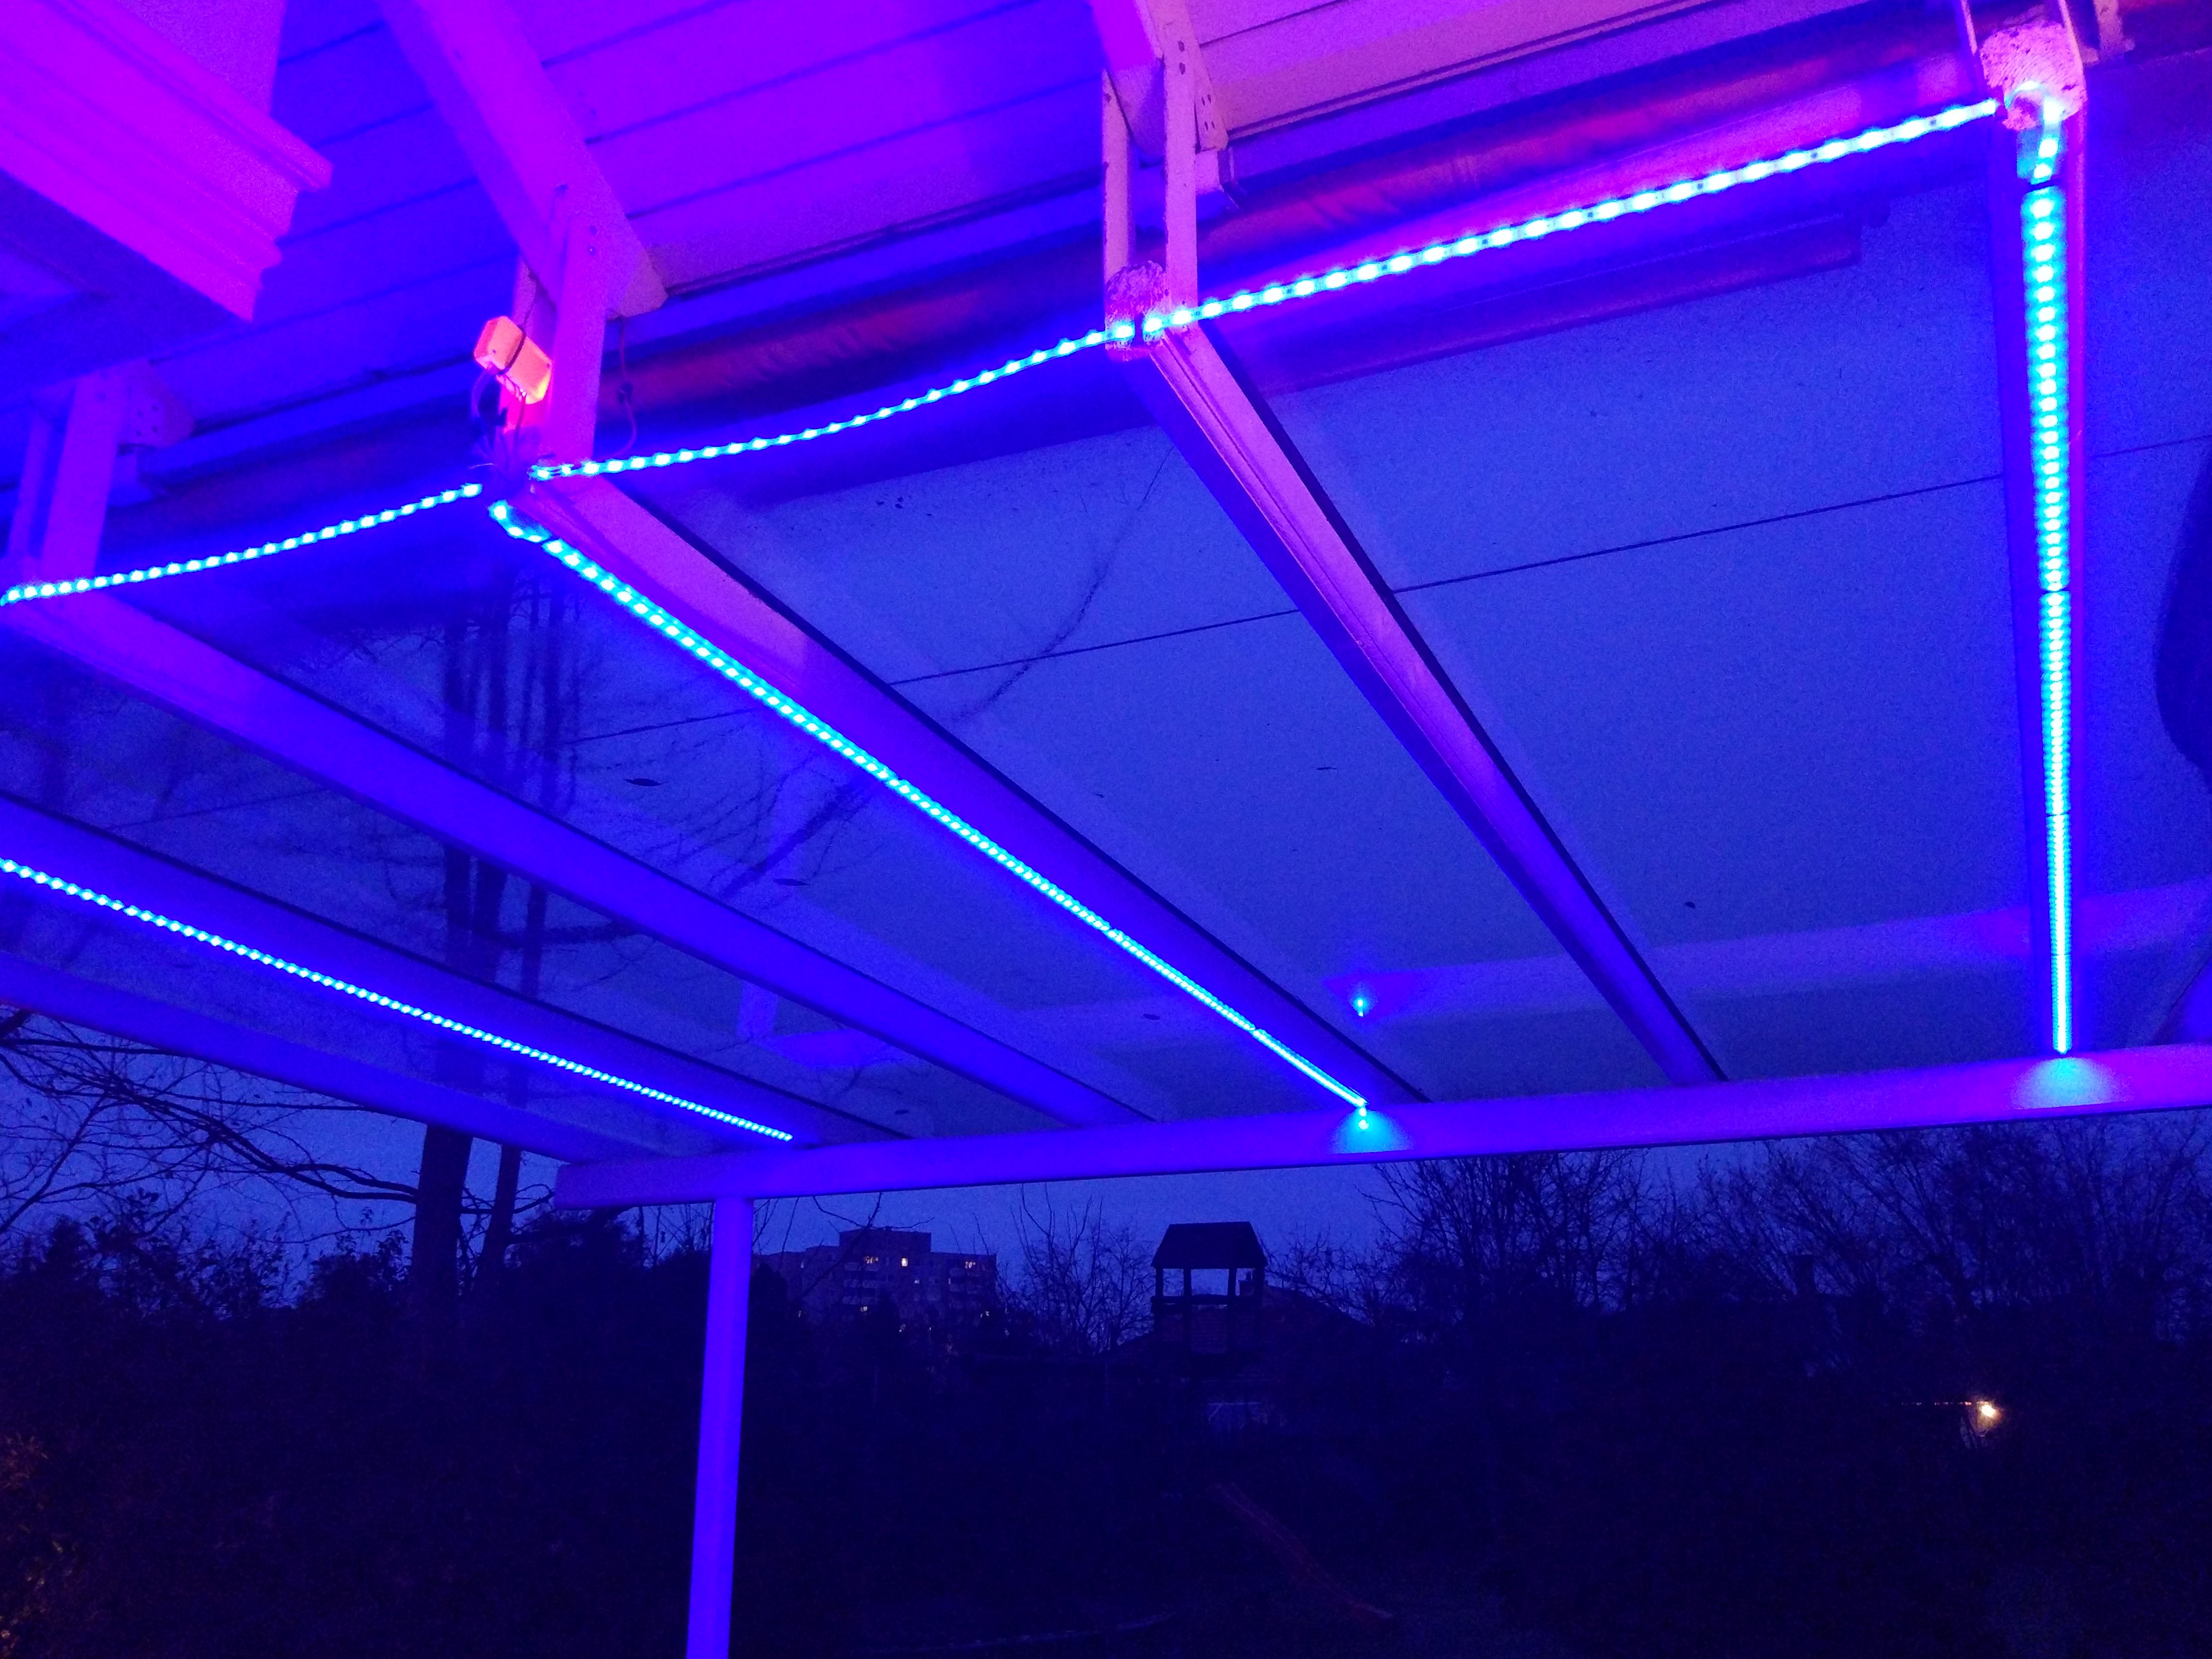
\includegraphics[height=3.8cm]{resources/alk_res/2_purpule_blue}
                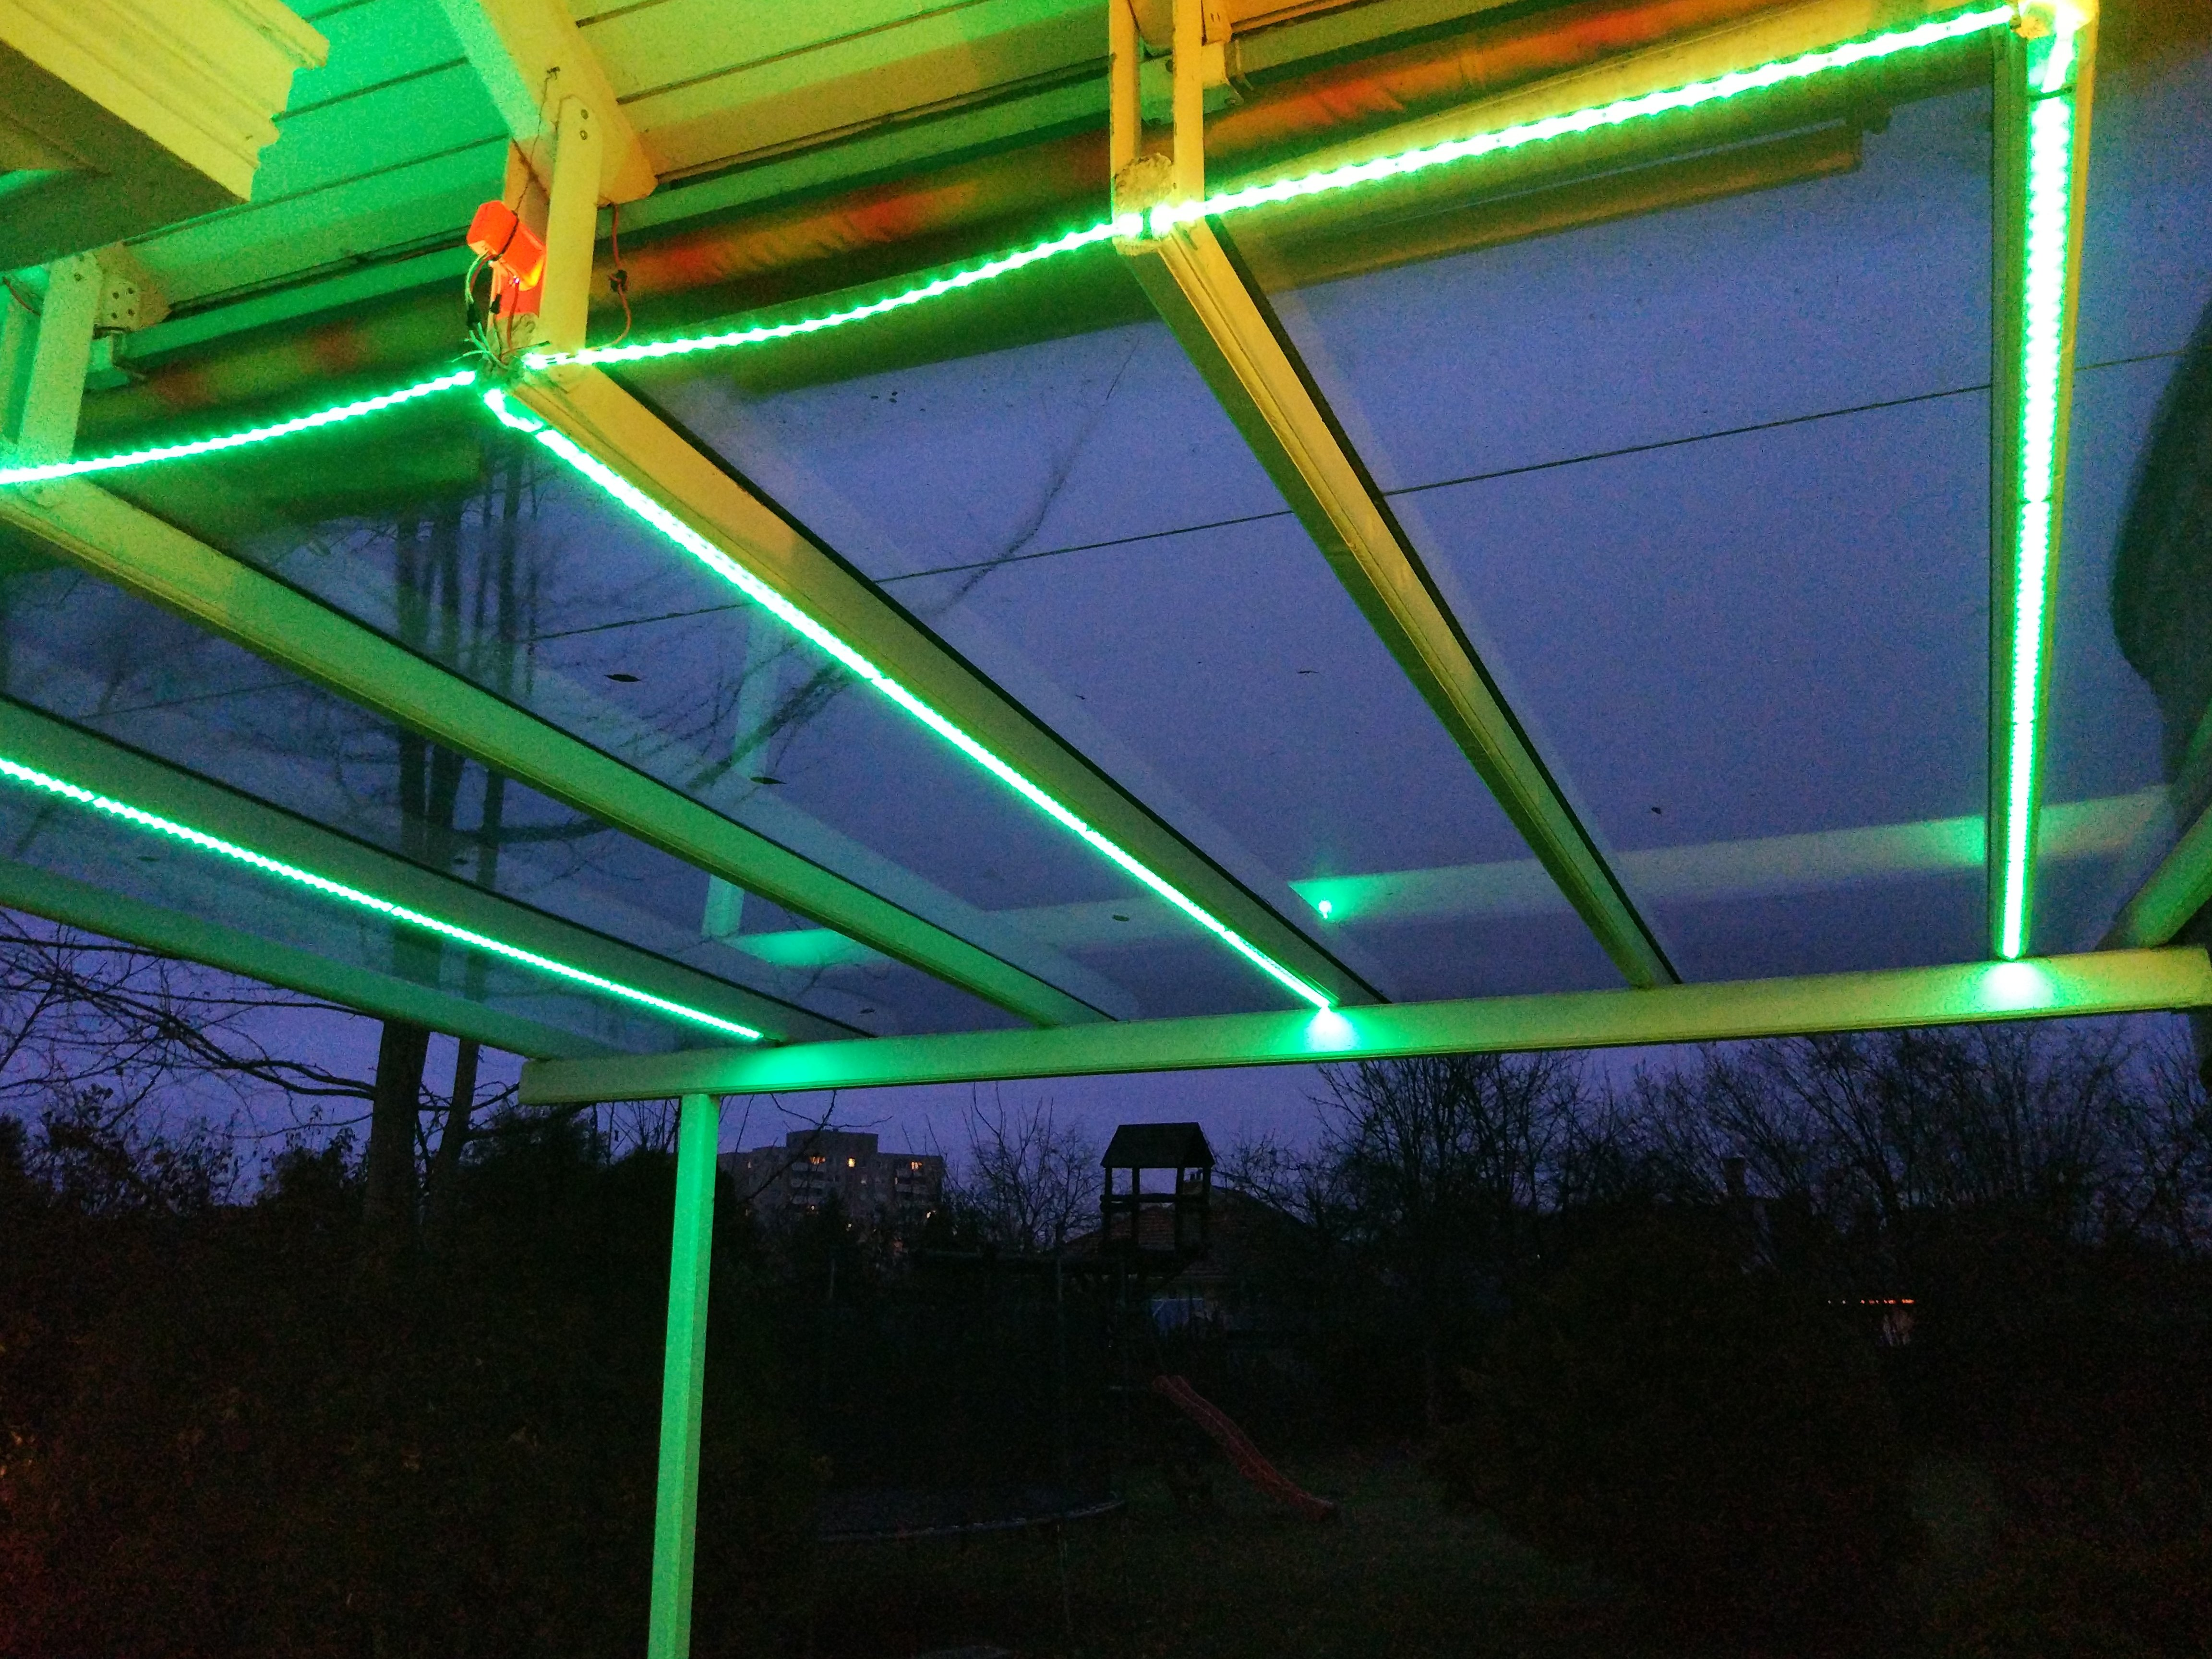
\includegraphics[height=3.8cm]{resources/alk_res/3_green}
                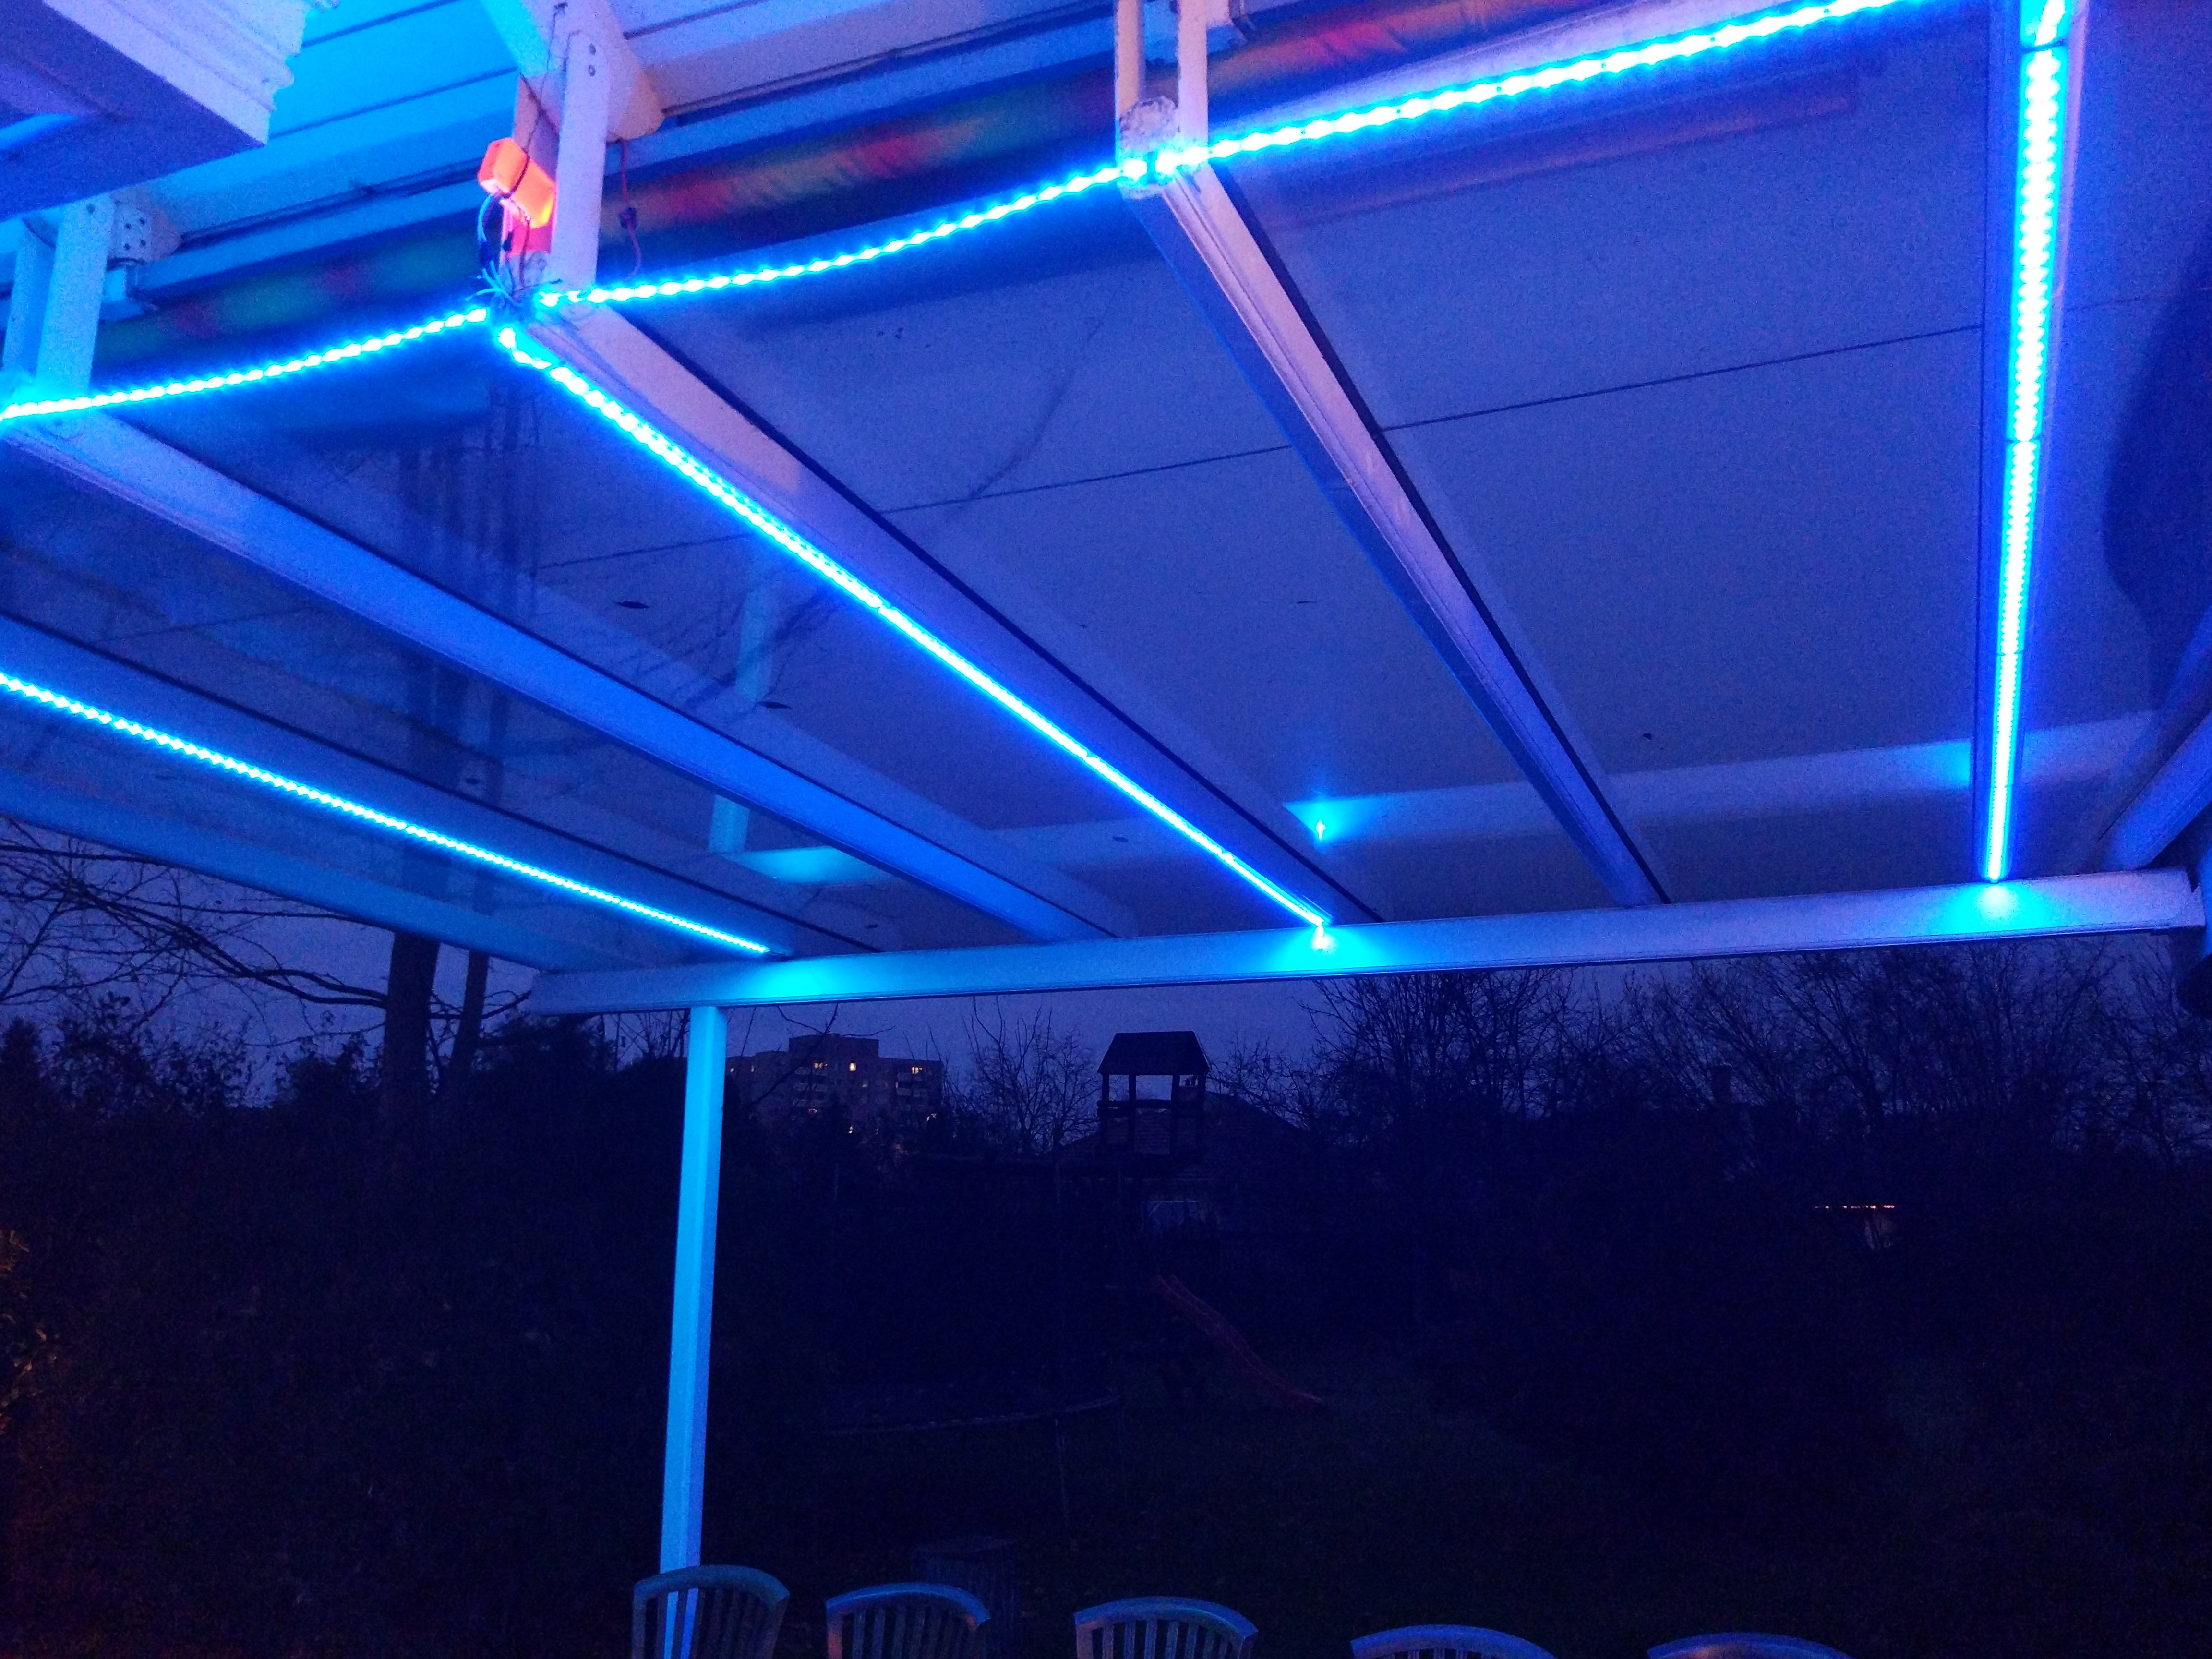
\includegraphics[height=3.8cm]{resources/alk_res/6_light_blue}
                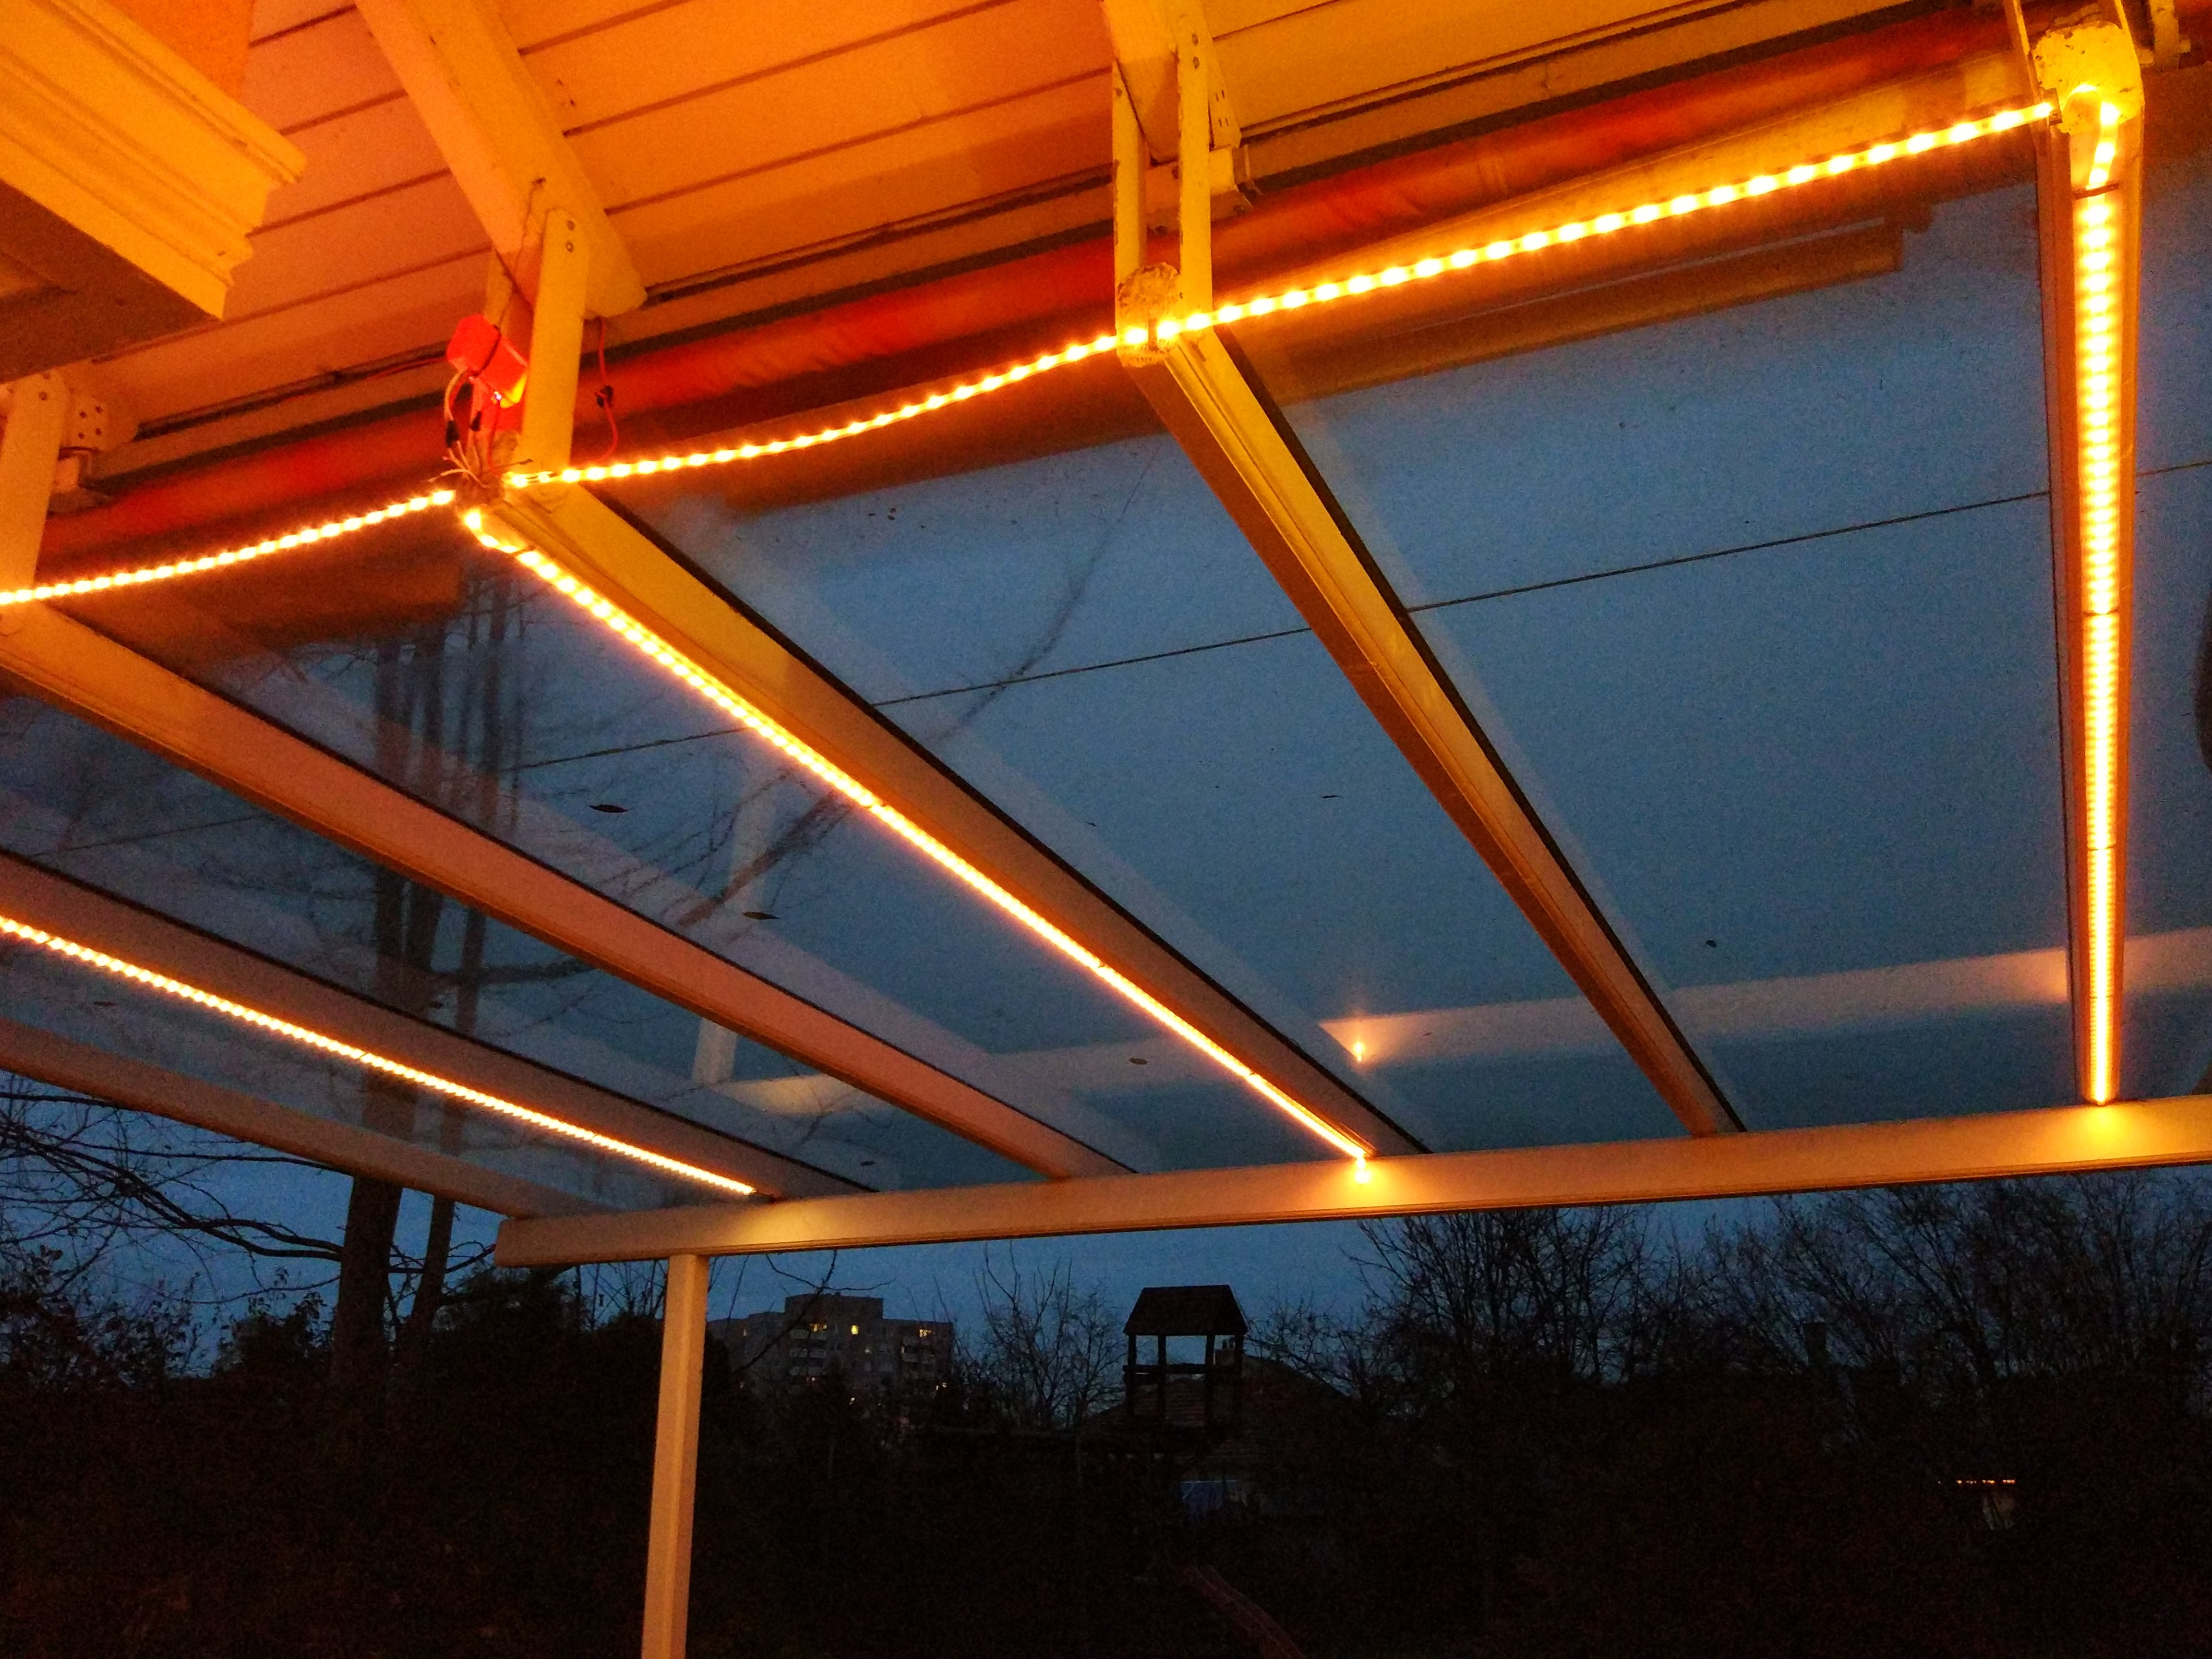
\includegraphics[height=3.8cm]{resources/alk_res/4_orange}
                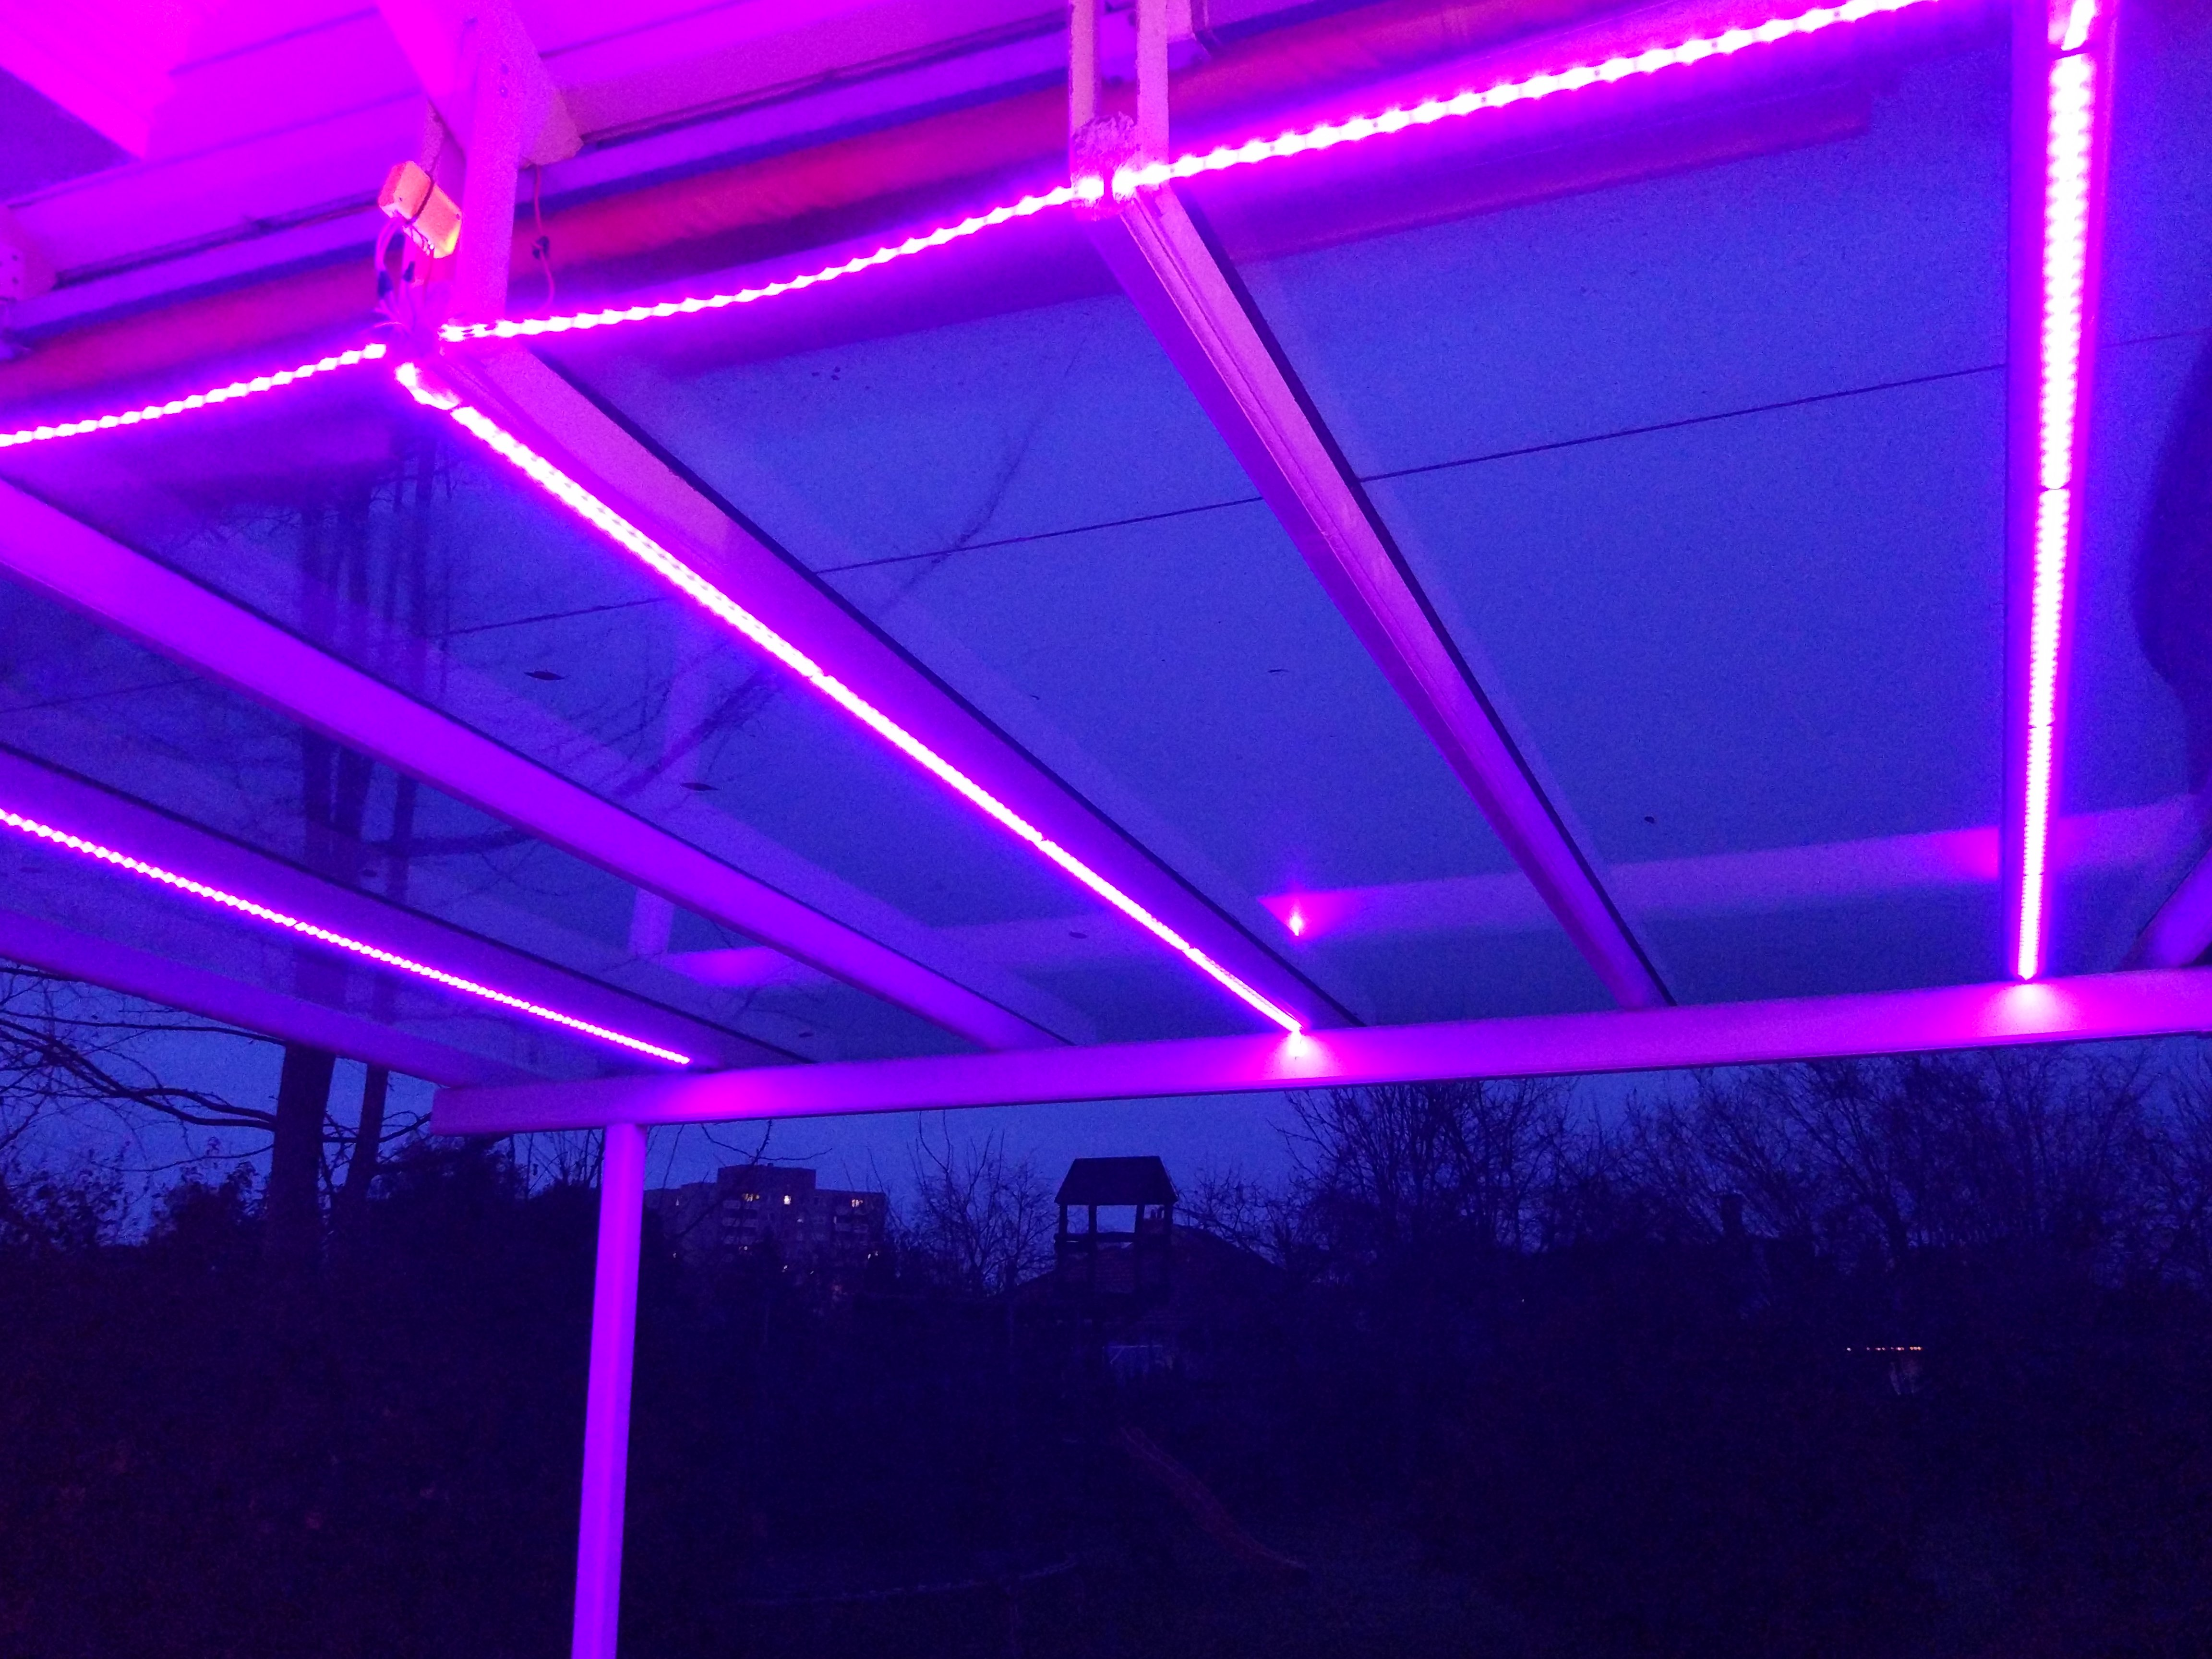
\includegraphics[height=3.8cm]{resources/alk_res/5_pink}
            \caption{Az elkészült eszköz különböző színeiben pompázva}
            \label{fig:pic_terasz}
        \end{figure}

    % \subsubsection{Összegzés az elvégzett munkáról}
        A feladat során megtanultam a Git verzió kezelő rendszer használatát, amivel többek között nyomon követhettem a haladási folyamatom.
        Elmélyítettem az objektumorientált Java, Android, illetve a hardverközeli C programozói tudásom is. Megtanultam a \textit{datasheet}-ek, \textit{reference manual}-ok, és \textit{application note}-ok segítségével megvalósítani beágyazott szoftvert. Megterveztem és legyártattam a LED sor vezérlő áramkörömet. Átismételtem, és kibővítettem paraméteres modellezési technikával a 3D-modellezési ismereteim.
        És végső soron új tapasztalatokat, ismereteket szereztem a forrasztás és a 3D nyomtatás területén. 
        
        % elmélyítettem mind az objektumorientált Java, illetve hardver közeli C programozói tudásom is. Átismételtem, és kibővítettem a 3D-modellezési ismereteim. Új tapasztalatokat, ismereteket szereztem a forrasztás és a 3D nyomtatás területén. 
        
        % A munkám tartalmazza az elektronikai tervezést, alkatrészek méretezését, a NYÁK legyártatását, az elektronikai komponensek beültetését, beforrasztását, ezek védelméül szolgáló doboz megtervezését, 3D nyomtatását, a beágyazott szoftver megírását, külső hardverrel való összekötését, illetve az egész rendszer vezérléséért felelős Android-os alkalmazást is.
    

    
    \subsection{Költségterv számolása}
        A költségtervbe csak az elkészült eszközök (3 db) alkatrész igényeit számoltam bele, illetve a működéshez szükséges perifériákat. Az feltüntetett árak csak körülbelüli értékek, illetve árfolyam függők.
        \begin{table}[h!]
        \centering
            \begin{tabular}{clrr}
            Darab     & Eszköz megnevezése                                      & Egységár  & Összesített ár \\
            \hline
            6         & 5m-es LED szalag                                        & 4500 Ft   & 27000 Ft       \\
            3         & 12V-os 5A-es egyenáramú áramforrás                      & 3300 Ft   & 9900 Ft        \\
            3         & ESP8266 Wifi modul                                      & 500 Ft    & 1500 Ft        \\
            1         & ST-Link V2 programozó                                   & 600 Ft    & 600 Ft         \\
            1         & 2x5 db NYÁK legyártása és szállítási díj                & 8500 Ft   & 8500 Ft        \\
            1         & Mouser Electronics-tól rendelt alkatrészek              & 22000 Ft  & 22000 Ft       \\
            3         & Védődoboz nyomtatása                                    & 1000 Ft   & 3000 Ft        \\
            1         & Extra kábelek, csatlakozók                              & 1500 Ft   & 1500 Ft        \\
            \hline
                      &                                                         & Összesen: & 74000 Ft      
            \end{tabular}
        \end{table}
        
        Három LED sor vezérlő legyártásához, vezérlőként két LED szalaggal, összesen 74000 Ft-ra van szükség. Tehát egy darab vezérlő egység (két LED sorral) körülbelül 25000 Ft-ba kerül. Ez az összeg már így is vetekszik a Philips és LIFX által forgalmazott eszközök áraival, de sorozatgyártással az ár tovább csökkenthető. A Mouser Electronics adataiból kiindulva, az árak 4000 darabos szériaszámnál a harmadára csökkennek, feltételezhetjük az összköltségünk is legalább a felére fog csökkenni.
    
    \subsection{Fejlesztési lehetőségek}
        Mind az beágyazott rendszer, mind az elkészült Android-os alkalmazáson nagyon sok mindent tovább lehetne fejleszteni, illetve rengetek plusz funkcióval ellátni. Első lépésben a kommunikációs protokoll továbbfejlesztésével kezdeném, hogy komplexebb szerkezetű adatokat, mint például új színpalettákat, lehessen küldeni a vezérlőegység számára.
        
        A beágyazott rendszer esetében fontosnak tartom egy erősebb mikrokontroller és egy mikrofon alkalmazását. Így nem kellene az Androidos alkalmazáson keresztül a zeneszámot Fourier transzformálni és 20-30 milliszekundumonként színeket küldözgetni a vezérlő egységnek, hanem saját magának számolná ki a szükséges adatokat. Ezzel jelentős mennyiségben lehetne a hálózati kommunikáció forgalmát csökkenteni és a telefon akkumulátoridejét növelni. A szoftvert fel lehetne készíteni komolyabb animációk megjelenítésére, folyamatok beütemezésére. Fejleszteni lehetne a zenére való színváltoztatást, kivilágosodást.
        
        Az Android-os applikációban biztosítani lehetne a különböző zeneszámok lejátszását. Ki lehetne bővíteni hangvezérléssel, és egy olyan nézettel, ahol a ledgroup csoportoknak, de akár egyesével is, lehetne változtatni a színét. Több nyelvű felhasználói felület megalkotása sem lenne utolsó szempont, az angolul nem tudó felhasználók számára. 
        
        % Az vezélőegység további perifériák, szenzorok alkalmazásával és az Internetre való csatlakoztatásával az IoT (Internet of Things) eszközök világába is becsatlakozna\cite{a_iot}.
        
\end{document}
